%%%%%%%%%%%%%%%%%%%%%%%%%%%%%%%%%%%%

\section{3.1. Distribuição normal}

%%%%%%%%%%%%%%%%%%%%%%%%%%%%%%%%%%%%

\begin{frame}
\frametitle{Distribuição normal}

\begin{itemize}
\justifying
\item Curva unimodal e simétrica em forma de sino
\justifying
\item Muitas variáveis são quase normais, mas nenhuma é exatamente normal
\justifying
\item Denotado como \mathhl{N(\mu,\sigma)} $\rightarrow$ Normal com média $\mu$ e desvio padrão $\sigma$

\end{itemize}

\begin{center}
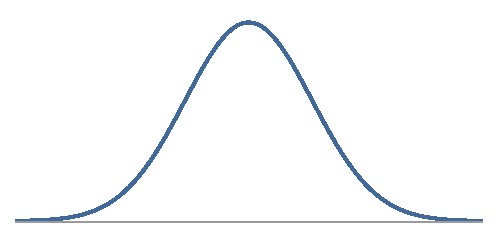
\includegraphics[width=0.7\textwidth]{3-1_normal_distribution/simpleNormal.pdf}
\end{center}

\end{frame}

%%%%%%%%%%%%%%%%%%%%%%%%%%%%%%%%%%%%

\begin{frame}
\frametitle{Alturas dos homens}

\twocol{0.5}{0.5}{
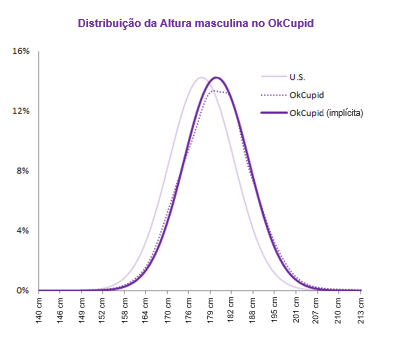
\includegraphics[width=\textwidth]{3-1_normal_distribution/ok_cupid_men.png} \\
}
{
\pause
\justifying
{\footnotesize \\ "As alturas dos homens no OkCupid quase seguem a distribuição normal esperada - exceto pelo fato de que o gráfico é mais deslocado para a direita do que na população geral de homens. Frequentemente os homens gostam de adicionar alguns centímetros à sua altura verdadeira." \\
\justifying
"Uma vaidade discreta pode ser observada: a parte superior da curva pontilhada, que começa em cerca de 176 cm, inclina-se ainda mais para a direita. Isso significa que eles chegam mais perto de um 1 metro e 80 cm, ou seja, aumentando ainda mais o valor de referência da altura desejada pelos homens."
}
}

\ct{\webURL{http://blog.okcupid.com/index.php/the-biggest-lies-in-online-dating/}}

\end{frame}

%%%%%%%%%%%%%%%%%%%%%%%%%%%%%%%%%%%%

\begin{frame}
\frametitle{Alturas das mulheres}

\twocol{0.5}{0.5}{
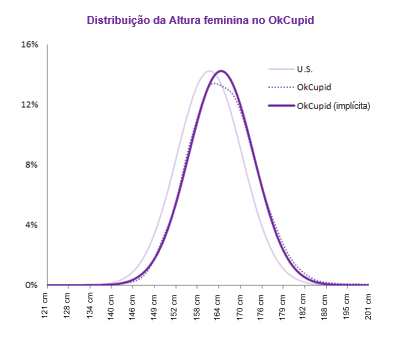
\includegraphics[width=\textwidth]{3-1_normal_distribution/ok_cupid_women.png} \\
}
{
\pause
\justifying
{\footnotesize \\" Já quando analisamos os dados das mulheres, ficamos surpresos ao ver que o exagero da altura uma característica tão propagada, embora, no caso das mulheres, sem necessariamente uma altura de referência desejada."
}
}

\vfill
\justifying
\ct{\webURL{http://blog.okcupid.com/index.php/the-biggest-lies-in-online-dating/}}

\end{frame}

%%%%%%%%%%%%%%%%%%%%%%%%%%%%%%%%%%%%

\subsection{Modelo de distribuição normal}

%%%%%%%%%%%%%%%%%%%%%%%%%%%%%%%%%%%%

\begin{frame}
\frametitle{Distribuições normais com diferentes parâmetros}

\vspace{-0.5cm}
\begin{center}
$\mu$: média, $\sigma$: desvio padrão
\[N(\mu = 0, \sigma = 1) \hspace{1.4cm} N(\mu = 19, \sigma = 4) \]
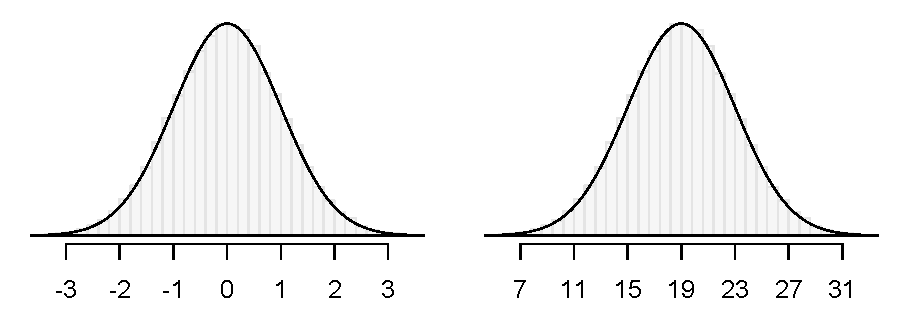
\includegraphics[width=0.6\textwidth]{3-1_normal_distribution/twoSampleNormals.pdf} \\
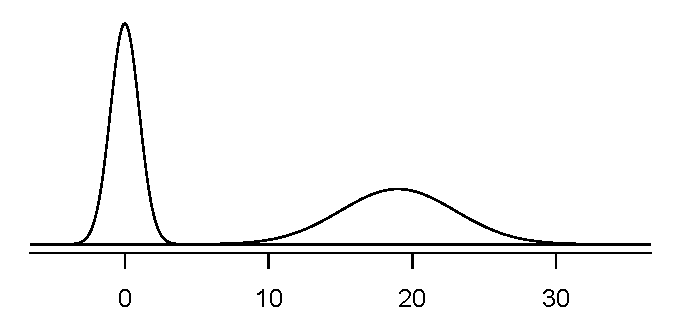
\includegraphics[width=0.6\textwidth]{3-1_normal_distribution/twoSampleNormalsStacked.pdf}
\end{center}

\end{frame}

%%%%%%%%%%%%%%%%%%%%%%%%%%%%%%%%%%%%

\subsection{Padronizando com escores Z}

%%%%%%%%%%%%%%%%%%%%%%%%%%%%%%%%%%%%

\begin{frame}
\frametitle{Distribuições normais com diferentes parâmetros}
\justifying
\dq{\footnotesize Os escores do SAT (\textit{Scholastic Aptitude Test} - um tipo de vestibular americano) possuem distribuição quase normal, com média 1.500 e desvio padrão 300. Os escores do ACT (\textit{American College Testing} - outro vestibular americano) também são distribuídos quase que normalmente, com média 21 e desvio padrão 5. 

\\ Um funcionário responsável pela aprovação dos candidatos em uma Universidade gostaria de determinar qual, de dois candidatos, obteve uma pontuação melhor em seu vestibular em relação aos outros vestibulandos: Pam, que obteve 1800 em seu SAT, ou Jim, que marcou 24 em seu ACT?}

\begin{center}
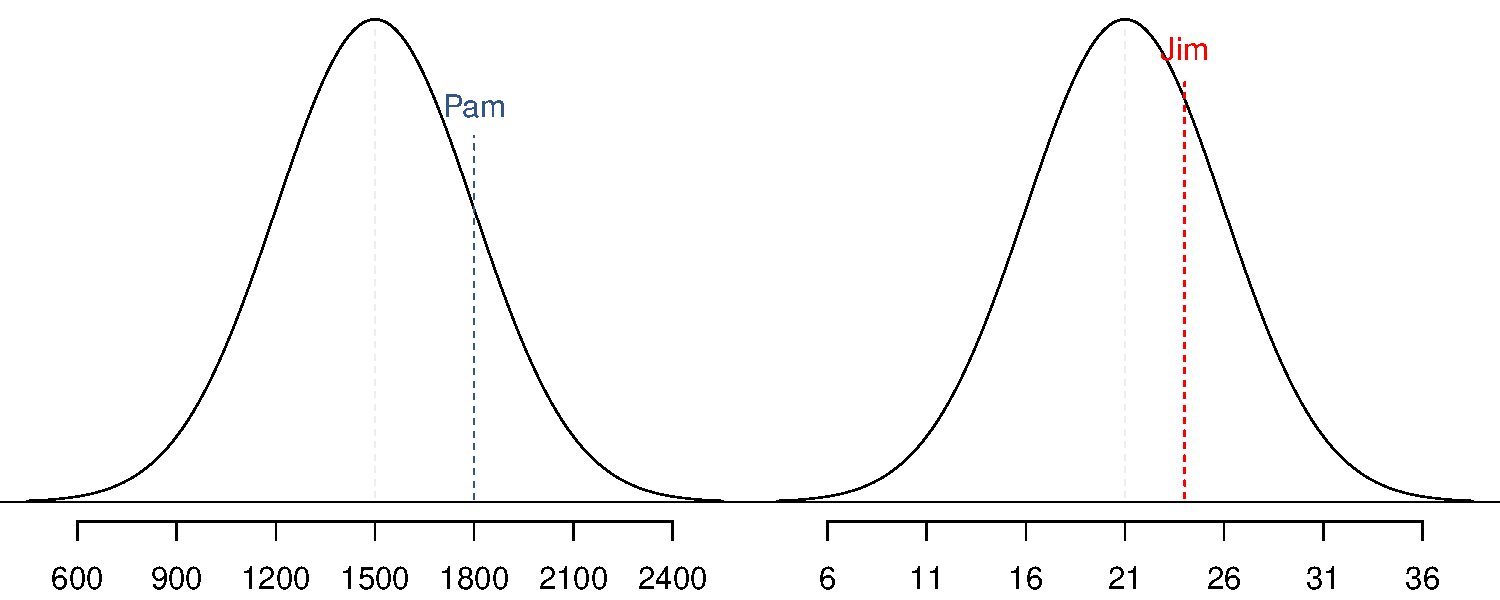
\includegraphics[width=0.8\textwidth]{3-1_normal_distribution/satActNormals.pdf}
\end{center}

\end{frame}

%%%%%%%%%%%%%%%%%%%%%%%%%%%%%%%%%%%%

\begin{frame}
\frametitle{Padronizando com escores Z}
\justifying
Como não podemos simplesmente comparar esses dois escores brutos, vamos verificar a quantos desvios-padrão além da média cada escore está.

\begin{itemize}
\justifying
\item A pontuação de Pam é $\frac{1800 - 1500}{300} = 1$ desvio padrão acima da média.
\justifying
\item A pontuação de Jim é $\frac{24 - 21}{5} = 0.6$ desvios-padrão acima da média.

\end{itemize}

\begin{center}
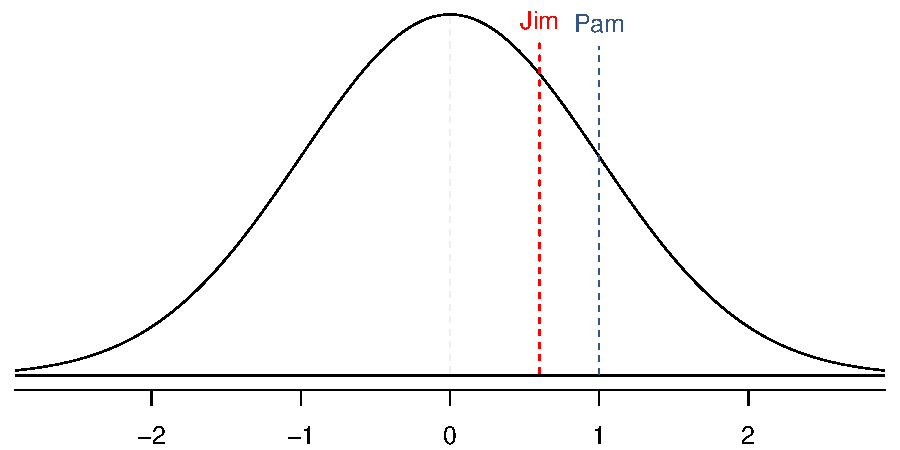
\includegraphics[width=0.6\textwidth]{3-1_normal_distribution/satActNormalsStandardized.pdf}
\end{center}

\end{frame}

%%%%%%%%%%%%%%%%%%%%%%%%%%%%%%%%%%%%

\begin{frame}
\frametitle{Padronizando com escores Z (cont.)}

\begin{itemize}
\justifying
\item Estes são chamados de \hl{escores padronizado}, ou \hl{escores Z}.
\justifying
\item O escore Z de uma observação é o número de desvios-padrão que esta observação está acima ou abaixo da média.\\
\formula{\[Z = \frac{observacao - media}{SD}\]}
\justifying
\item Os escores Z são definidos para distribuições de qualquer formato, porém somente quando a distribuição é normal podemos usar escores Z para calcular \hl{percentis}.
\justifying
\item Observações que estão a mais de 2 desvios-padrão da média ($ | Z |> 2 $) são geralmente consideradas incomuns.

\end{itemize}

\end{frame}

%%%%%%%%%%%%%%%%%%%%%%%%%%%%%%%%%%%%

\begin{frame}
\frametitle{Percentis}

\begin{itemize}
\justifying
\item \hl{Percentil} é a porcentagem de observações que caem abaixo de um determinado valor da distribuição de dados.
\justifying
\item Graficamente, o percentil é a área abaixo da curva de distribuição de probabilidade à esquerda dessa observação.

\end{itemize}

\begin{center}
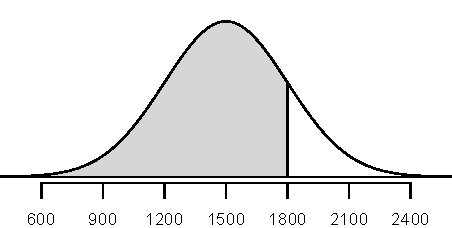
\includegraphics[width=0.7\textwidth]{3-1_normal_distribution/satBelow1800.pdf}
\end{center}

\end{frame}

%%%%%%%%%%%%%%%%%%%%%%%%%%%%%%%%%%%%

\begin{frame}
\frametitle{Percentis}
\justifying
\dq{Aproximadamente, qual porcentagem de alunos tem pontuação abaixo de 1800 no SAT? (Dica: use a regra 68-95-99.7\%.)}

\only<1>{
\begin{center}
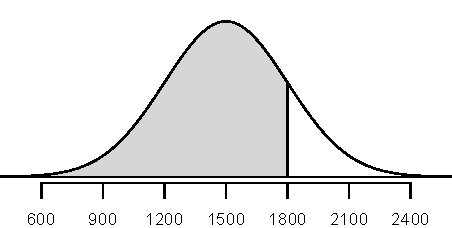
\includegraphics[width=0.7\textwidth]{3-1_normal_distribution/satBelow1800.pdf}
\end{center}
}

\only<2 | handout:0>{
\begin{center}
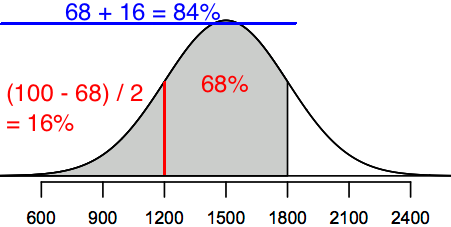
\includegraphics[width=0.7\textwidth]{3-1_normal_distribution/satBelow1800_soln.png}
\end{center}
}
\vspace{-0.5cm}
\soln{\only<2>{
\begin{align*}
100 - 68 &= 32\% \\
32 / 2 &= 16\% \\
68 + 16 &= 84\%
\end{align*}}}

\end{frame}
%
%%%%%%%%%%%%%%%%%%%%%%%%%%%%%%%%%%%%%

\subsection{Tabela de probabilidade normal}

%%%%%%%%%%%%%%%%%%%%%%%%%%%%%%%%%%%%

\begin{frame}[fragile]
\frametitle{Calculando percentis - usando computação}
\justifying
Existem muitas maneiras de calcular os percentis/áreas sob a curva:

\begin{itemize}
\item R:
\end{itemize}
\begin{beamerboxesrounded}[shadow = false, lower = code body]{}
{\small \begin{verbatim}
> pnorm(1800, mean = 1500, sd = 300)
[1] 0.8413447
\end{verbatim}
}
\end{beamerboxesrounded}
\begin{itemize}
\item Applet: {\small \webURL{https://gallery.shinyapps.io/dist_calc/}}
\begin{center}
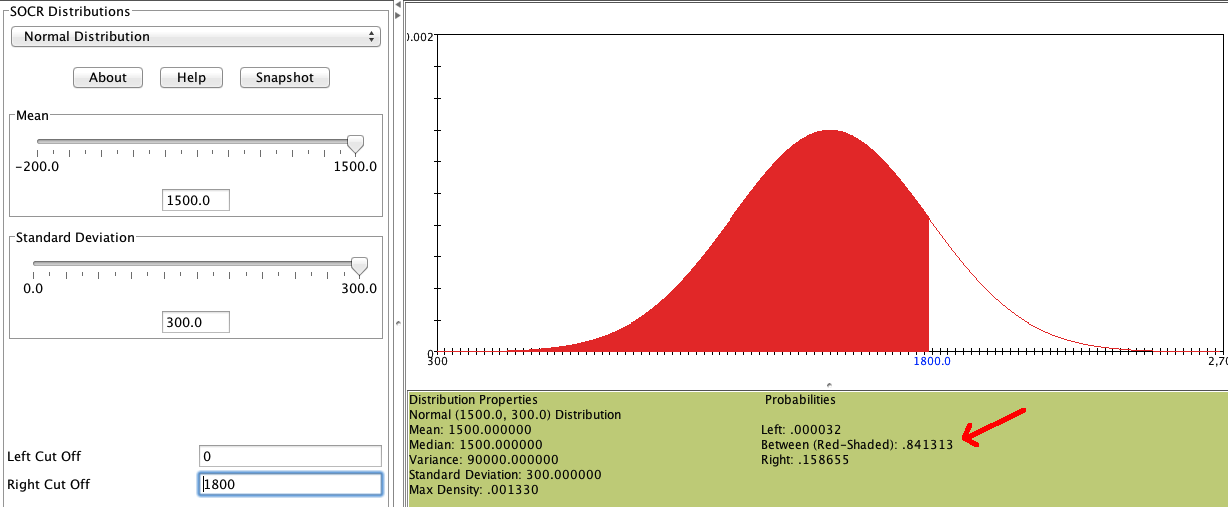
\includegraphics[width=0.8\textwidth]{3-1_normal_distribution/applet.png}
\end{center}

\end{itemize}


\end{frame}

%%%%%%%%%%%%%%%%%%%%%%%%%%%%%%%%%%%%

\begin{frame}[fragile]
\frametitle{Calculando percentis - usando tabelas}

{\footnotesize
\begin{tabular}{c | >{\columncolor[gray]{0.6}[0pt]}rrrrr | rrrrr |}
  \cline{2-11}
&&&& \multicolumn{4}{c}{Second decimal place of $Z$} &&& \\
  \cline{2-11}
$Z$ & 0.00 & 0.01 & 0.02 & 0.03 & 0.04 & 0.05 & 0.06 & 0.07 & 0.08 & 0.09 \\
  \hline
  \hline
0.0 & \tiny{0.5000} & \tiny{0.5040} & \tiny{0.5080} & \tiny{0.5120} & \tiny{0.5160} & \tiny{0.5199} & \tiny{0.5239} & \tiny{0.5279} & \tiny{0.5319} & \tiny{0.5359} \\
  0.1 & \tiny{0.5398} & \tiny{0.5438} & \tiny{0.5478} & \tiny{0.5517} & \tiny{0.5557} & \tiny{0.5596} & \tiny{0.5636} & \tiny{0.5675} & \tiny{0.5714} & \tiny{0.5753} \\
  0.2 & \tiny{0.5793} & \tiny{0.5832} & \tiny{0.5871} & \tiny{0.5910} & \tiny{0.5948} & \tiny{0.5987} & \tiny{0.6026} & \tiny{0.6064} & \tiny{0.6103} & \tiny{0.6141} \\
  0.3 & \tiny{0.6179} & \tiny{0.6217} & \tiny{0.6255} & \tiny{0.6293} & \tiny{0.6331} & \tiny{0.6368} & \tiny{0.6406} & \tiny{0.6443} & \tiny{0.6480} & \tiny{0.6517} \\
  0.4 & \tiny{0.6554} & \tiny{0.6591} & \tiny{0.6628} & \tiny{0.6664} & \tiny{0.6700} & \tiny{0.6736} & \tiny{0.6772} & \tiny{0.6808} & \tiny{0.6844} & \tiny{0.6879} \\
  \hline
  0.5 & \tiny{0.6915} & \tiny{0.6950} & \tiny{0.6985} & \tiny{0.7019} & \tiny{0.7054} & \tiny{0.7088} & \tiny{0.7123} & \tiny{0.7157} & \tiny{0.7190} & \tiny{0.7224} \\
  0.6 & \tiny{0.7257} & \tiny{0.7291} & \tiny{0.7324} & \tiny{0.7357} & \tiny{0.7389} & \tiny{0.7422} & \tiny{0.7454} & \tiny{0.7486} & \tiny{0.7517} & \tiny{0.7549} \\
  0.7 & \tiny{0.7580} & \tiny{0.7611} & \tiny{0.7642} & \tiny{0.7673} & \tiny{0.7704} & \tiny{0.7734} & \tiny{0.7764} & \tiny{0.7794} & \tiny{0.7823} & \tiny{0.7852} \\
  0.8 & \tiny{0.7881} & \tiny{0.7910} & \tiny{0.7939} & \tiny{0.7967} & \tiny{0.7995} & \tiny{0.8023} & \tiny{0.8051} & \tiny{0.8078} & \tiny{0.8106} & \tiny{0.8133} \\
  0.9 & \tiny{0.8159} & \tiny{0.8186} & \tiny{0.8212} & \tiny{0.8238} & \tiny{0.8264} & \tiny{0.8289} & \tiny{0.8315} & \tiny{0.8340} & \tiny{0.8365} & \tiny{0.8389} \\
  \hline
  \hline
\rowcolor[gray]{.6}
  1.0 & \orange{\tiny{0.8413}} & \tiny{0.8438} & \tiny{0.8461} & \tiny{0.8485} & \tiny{0.8508} & \tiny{0.8531} & \tiny{0.8554} & \tiny{0.8577} & \tiny{0.8599} & \tiny{0.8621} \\
  1.1 & \tiny{0.8643} & \tiny{0.8665} & \tiny{0.8686} & \tiny{0.8708} & \tiny{0.8729} & \tiny{0.8749} & \tiny{0.8770} & \tiny{0.8790} & \tiny{0.8810} & \tiny{0.8830} \\
  1.2 & \tiny{0.8849} & \tiny{0.8869} & \tiny{0.8888} & \tiny{0.8907} & \tiny{0.8925} & \tiny{0.8944} & \tiny{0.8962} & \tiny{0.8980} & \tiny{0.8997} & \tiny{0.9015} \\
\end{tabular}
}

\end{frame}

%%%%%%%%%%%%%%%%%%%%%%%%%%%%%%%%%%%%

\subsection{Exemplos de probabilidade normal}

%%%%%%%%%%%%%%%%%%%%%%%%%%%%%%%%%%%%

\begin{frame}
\frametitle{6 sigma}
\justifying
``O termo \textit {processo 6 sigma} vem da ideia de que, se houver seis desvios-padrão entre a média do processo e o limite de especificação mais próximo, como mostrado no gráfico, praticamente nenhum item deixará de atender às especificações."

\begin{center}
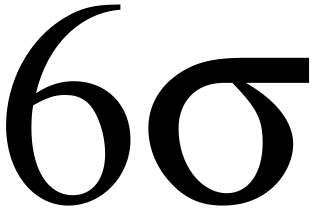
\includegraphics[width=0.35\textwidth]{3-1_normal_distribution/sixsigma.png}
\end{center}

\ct{\webURL{http://en.wikipedia.org/wiki/Six_Sigma}}

\end{frame}

%%%%%%%%%%%%%%%%%%%%%%%%%%%%%%%%%%%%

\begin{frame}
\frametitle{Controle de qualidade}
\justifying
\dq{{\small Na fábrica de ketchup Heinz, as quantidades de ketchup inseridas nas garrafas devem ser normalmente distribuídas com uma média de 36g e desvio-padrão 0,11g. A cada 30 minutos, uma garrafa é selecionada da linha de produção e seu conteúdo é precisamente anotado. Se a quantidade de ketchup na garrafa estiver abaixo de 35,8g ou acima de 36,2g, então o frasco falha na inspeção de controle de qualidade. Qual a porcentagem de garrafas possue menos de 35,8g de ketchup?}}

\soln{\pause
\centering Seja $X$ = quantidade de ketchup em uma garrafa: \\ $X \sim N(\mu = 36, \sigma = 0,11)$ \\
\pause
\twocol{0.4}{0.6}{
\begin{center}
\centering
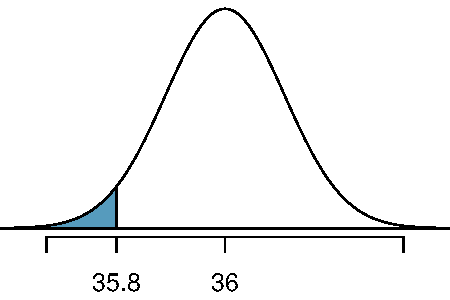
\includegraphics[width=\textwidth]{3-1_normal_distribution/ketchupLT358.pdf}
\end{center}
}
{
\pause
\[ Z = \frac{35.8 - 36}{0.11} = -1.82 \]
}
}

\end{frame}

%%%%%%%%%%%%%%%%%%%%%%%%%%%%%%%%%%%%

\begin{frame}
\frametitle{Encontrar a probabilidade exata - usando a tabela Z}

\only<1>{
{\footnotesize
\begin{tabular}{| rrrrr | rrrrr | c}
  \cline{1-10}
&&& \multicolumn{4}{c}{Segunda casa decimal de $ Z $} &&& \\
  \cline{1-10}
0.09 &  0.08 &  0.07 &  0.06 &  0.05 &  0.04 &  0.03 &  0.02 &  0.01 &  0.00 & $Z$  \\
    \hline
    \hline
  \tiny{0.0014} & \tiny{0.0014} & \tiny{0.0015} & \tiny{0.0015} & \tiny{0.0016} & \tiny{0.0016} & \tiny{0.0017} & \tiny{0.0018} & \tiny{0.0018} & \tiny{0.0019} & $-2.9$ \\
  \tiny{0.0019} & \tiny{0.0020} & \tiny{0.0021} & \tiny{0.0021} & \tiny{0.0022} & \tiny{0.0023} & \tiny{0.0023} & \tiny{0.0024} & \tiny{0.0025} & \tiny{0.0026} & $-2.8$ \\
  \tiny{0.0026} & \tiny{0.0027} & \tiny{0.0028} & \tiny{0.0029} & \tiny{0.0030} & \tiny{0.0031} & \tiny{0.0032} & \tiny{0.0033} & \tiny{0.0034} & \tiny{0.0035} & $-2.7$ \\
  \tiny{0.0036} & \tiny{0.0037} & \tiny{0.0038} & \tiny{0.0039} & \tiny{0.0040} & \tiny{0.0041} & \tiny{0.0043} & \tiny{0.0044} & \tiny{0.0045} & \tiny{0.0047} & $-2.6$ \\
  \tiny{0.0048} & \tiny{0.0049} & \tiny{0.0051} & \tiny{0.0052} & \tiny{0.0054} & \tiny{0.0055} & \tiny{0.0057} & \tiny{0.0059} & \tiny{0.0060} & \tiny{0.0062} & $-2.5$ \\
    \hline
  \tiny{0.0064} & \tiny{0.0066} & \tiny{0.0068} & \tiny{0.0069} & \tiny{0.0071} & \tiny{0.0073} & \tiny{0.0075} & \tiny{0.0078} & \tiny{0.0080} & \tiny{0.0082} & $-2.4$ \\
  \tiny{0.0084} & \tiny{0.0087} & \tiny{0.0089} & \tiny{0.0091} & \tiny{0.0094} & \tiny{0.0096} & \tiny{0.0099} & \tiny{0.0102} & \tiny{0.0104} & \tiny{0.0107} & $-2.3$ \\
  \tiny{0.0110} & \tiny{0.0113} & \tiny{0.0116} & \tiny{0.0119} & \tiny{0.0122} & \tiny{0.0125} & \tiny{0.0129} & \tiny{0.0132} & \tiny{0.0136} & \tiny{0.0139} & $-2.2$ \\
  \tiny{0.0143} & \tiny{0.0146} & \tiny{0.0150} & \tiny{0.0154} & \tiny{0.0158} & \tiny{0.0162} & \tiny{0.0166} & \tiny{0.0170} & \tiny{0.0174} & \tiny{0.0179} & $-2.1$ \\
  \tiny{0.0183} & \tiny{0.0188} & \tiny{0.0192} & \tiny{0.0197} & \tiny{0.0202} & \tiny{0.0207} & \tiny{0.0212} & \tiny{0.0217} & \tiny{0.0222} & \tiny{0.0228} & $-2.0$ \\
    \hline
  \tiny{0.0233} & \tiny{0.0239} & \tiny{0.0244} & \tiny{0.0250} & \tiny{0.0256} & \tiny{0.0262} & \tiny{0.0268} & \tiny{0.0274} & \tiny{0.0281} & \tiny{0.0287} & $-1.9$ \\
  \tiny{0.0294} & \tiny{0.0301} & \tiny{0.0307} & \tiny{0.0314} & \tiny{0.0322} & \tiny{0.0329} & \tiny{0.0336} & \tiny{0.0344} & \tiny{0.0351} & \tiny{0.0359} & $-1.8$ \\
  \tiny{0.0367} & \tiny{0.0375} & \tiny{0.0384} & \tiny{0.0392} & \tiny{0.0401} & \tiny{0.0409} & \tiny{0.0418} & \tiny{0.0427} & \tiny{0.0436} & \tiny{0.0446} & $-1.7$ \\
  \tiny{0.0455} & \tiny{0.0465} & \tiny{0.0475} & \tiny{0.0485} & \tiny{0.0495} & \tiny{0.0505} & \tiny{0.0516} & \tiny{0.0526} & \tiny{0.0537} & \tiny{0.0548} & $-1.6$ \\
  \tiny{0.0559} & \tiny{0.0571} & \tiny{0.0582} & \tiny{0.0594} & \tiny{0.0606} & \tiny{0.0618} & \tiny{0.0630} & \tiny{0.0643} & \tiny{0.0655} & \tiny{0.0668} & $-1.5$ \\
\hline
\end{tabular}
}}

\soln{
\only<2|folheto:0>{
{\scalefont{0.6}
\begin{tabular}{| rrrrr | rr>{\columncolor[gray]{0.6}[0pt]}rrr | c}
  \cline{1-10}
&&& \multicolumn{4}{c}{Segunda casa decimal de $ Z $} &&& \\
  \cline{1-10}
0.09 &  0.08 &  0.07 &  0.06 &  0.05 &  0.04 &  0.03 &  0.02 &  0.01 &  0.00 & $Z$  \\
    \hline
    \hline
  \tiny{0.0014} & \tiny{0.0014} & \tiny{0.0015} & \tiny{0.0015} & \tiny{0.0016} & \tiny{0.0016} & \tiny{0.0017} & \tiny{0.0018} & \tiny{0.0018} & \tiny{0.0019} & $-2.9$ \\
  \tiny{0.0019} & \tiny{0.0020} & \tiny{0.0021} & \tiny{0.0021} & \tiny{0.0022} & \tiny{0.0023} & \tiny{0.0023} & \tiny{0.0024} & \tiny{0.0025} & \tiny{0.0026} & $-2.8$ \\
  \tiny{0.0026} & \tiny{0.0027} & \tiny{0.0028} & \tiny{0.0029} & \tiny{0.0030} & \tiny{0.0031} & \tiny{0.0032} & \tiny{0.0033} & \tiny{0.0034} & \tiny{0.0035} & $-2.7$ \\
  \tiny{0.0036} & \tiny{0.0037} & \tiny{0.0038} & \tiny{0.0039} & \tiny{0.0040} & \tiny{0.0041} & \tiny{0.0043} & \tiny{0.0044} & \tiny{0.0045} & \tiny{0.0047} & $-2.6$ \\
  \tiny{0.0048} & \tiny{0.0049} & \tiny{0.0051} & \tiny{0.0052} & \tiny{0.0054} & \tiny{0.0055} & \tiny{0.0057} & \tiny{0.0059} & \tiny{0.0060} & \tiny{0.0062} & $-2.5$ \\
    \hline
  \tiny{0.0064} & \tiny{0.0066} & \tiny{0.0068} & \tiny{0.0069} & \tiny{0.0071} & \tiny{0.0073} & \tiny{0.0075} & \tiny{0.0078} & \tiny{0.0080} & \tiny{0.0082} & $-2.4$ \\
  \tiny{0.0084} & \tiny{0.0087} & \tiny{0.0089} & \tiny{0.0091} & \tiny{0.0094} & \tiny{0.0096} & \tiny{0.0099} & \tiny{0.0102} & \tiny{0.0104} & \tiny{0.0107} & $-2.3$ \\
  \tiny{0.0110} & \tiny{0.0113} & \tiny{0.0116} & \tiny{0.0119} & \tiny{0.0122} & \tiny{0.0125} & \tiny{0.0129} & \tiny{0.0132} & \tiny{0.0136} & \tiny{0.0139} & $-2.2$ \\
  \tiny{0.0143} & \tiny{0.0146} & \tiny{0.0150} & \tiny{0.0154} & \tiny{0.0158} & \tiny{0.0162} & \tiny{0.0166} & \tiny{0.0170} & \tiny{0.0174} & \tiny{0.0179} & $-2.1$ \\
  \tiny{0.0183} & \tiny{0.0188} & \tiny{0.0192} & \tiny{0.0197} & \tiny{0.0202} & \tiny{0.0207} & \tiny{0.0212} & \tiny{0.0217} & \tiny{0.0222} & \tiny{0.0228} & $-2.0$ \\
    \hline
  \tiny{0.0233} & \tiny{0.0239} & \tiny{0.0244} & \tiny{0.0250} & \tiny{0.0256} & \tiny{0.0262} & \tiny{0.0268} & \tiny{0.0274} & \tiny{0.0281} & \tiny{0.0287} & $-1.9$ \\
\rowcolor[gray]{.6}
  \tiny{0.0294} & \tiny{0.0301} & \tiny{0.0307} & \tiny{0.0314} & \tiny{0.0322} & \tiny{0.0329} & \tiny{0.0336} & \orange{\tiny{0.0344}} & \tiny{0.0351} & \tiny{0.0359} & $-1.8$ \\
  \tiny{0.0367} & \tiny{0.0375} & \tiny{0.0384} & \tiny{0.0392} & \tiny{0.0401} & \tiny{0.0409} & \tiny{0.0418} & \tiny{0.0427} & \tiny{0.0436} & \tiny{0.0446} & $-1.7$ \\
  \tiny{0.0455} & \tiny{0.0465} & \tiny{0.0475} & \tiny{0.0485} & \tiny{0.0495} & \tiny{0.0505} & \tiny{0.0516} & \tiny{0.0526} & \tiny{0.0537} & \tiny{0.0548} & $-1.6$ \\
  \tiny{0.0559} & \tiny{0.0571} & \tiny{0.0582} & \tiny{0.0594} & \tiny{0.0606} & \tiny{0.0618} & \tiny{0.0630} & \tiny{0.0643} & \tiny{0.0655} & \tiny{0.0668} & $-1.5$ \\
\hline
\end{tabular}
}}}

\end{frame}

%%%%%%%%%%%%%%%%%%%%%%%%%%%%%%%%%%%%

\begin{frame}[fragile]
\frametitle{Encontrar a probabilidade exata - usando R}

\begin{beamerboxesrounded}[shadow = true, lower = code body]{}
{\small \begin{verbatim}
> pnorm(-1.82, mean = 0, sd = 1)
[1] 0.0344
\end{verbatim}
}
\end{beamerboxesrounded}

$\:$ \\
\pause

ou

$\:$ \\
\pause

\begin{beamerboxesrounded}[shadow = true, lower = code body]{}
{\small \begin{verbatim}
> pnorm(35.8, mean = 36, sd = 0.11)
[1] 0.0345
\end{verbatim}
}
\end{beamerboxesrounded}


\end{frame}
%
%%%%%%%%%%%%%%%%%%%%%%%%%%%%%%%%%%%%%

\begin{frame}
\frametitle{Prática}
\justifying
\pq{Qual o percentual de garrafas que \underline {passa} na inspeção de controle de qualidade?}

\vspace{-0.5cm}
\begin{multicols}{2}
\begin{enumerate}[(a)]
\item 1.82\%
\item 3.44\%
\item 6.88\%
\solnMult{93.12\%}
\item 96.56\%
\item[]
\end{enumerate}
\end{multicols}

\soln{
\vspace{-0.5cm}
\pause
\begin{columns}[c]
\column{0.3\textwidth}
\pause
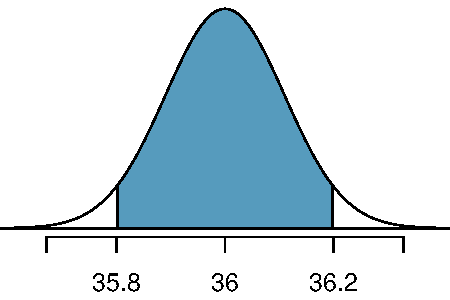
\includegraphics[width=\textwidth]{3-1_normal_distribution/ketchupBET.pdf}
\column{0.05\textwidth}
=
\pause
\column{0.3\textwidth}
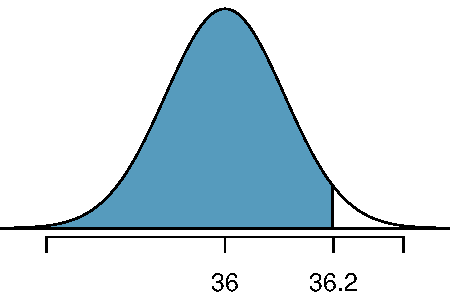
\includegraphics[width=\textwidth]{3-1_normal_distribution/ketchupLT362.pdf}
\column{0.05\textwidth}
-
\pause
\column{0.3\textwidth}
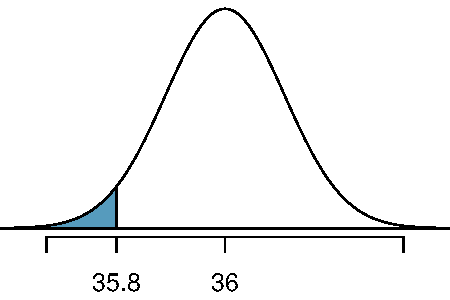
\includegraphics[width=\textwidth]{3-1_normal_distribution/ketchupLT358.pdf}
\end{columns}
\pause
\scalefont{0.8}
\begin{eqnarray*}
Z_{35.8} &=& \frac{35.8 - 36}{0.11} = -1.82 \\ \pause
Z_{36.2} &=& \frac{36.2 - 36}{0.11} = 1.82 \\ \pause
P(35.8 < X < 36.2) &=& P(-1.82 < Z < 1.82) = 0.9656 - 0.0344 = 0.9312
\end{eqnarray*}
}

\end{frame}

%%%%%%%%%%%%%%%%%%%%%%%%%%%%%%%%%%%%

\begin{frame}
\frametitle{Encontrando pontos de corte}
\justifying
\dq{\footnotesize Em seres humanos saudáveis, as temperaturas corporais são distribuídas quase que normalmente com média 98,2$^{\circ}$ F e desvio-padrão de 0,73$^{\circ}$ F. \\ Qual é o ponto de corte dos 3\% que possuem temperaturas corporais mais baixas?}

\pause

\twocol{0.35}{0.65}
{
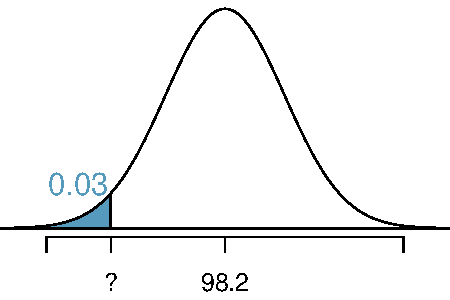
\includegraphics[width=\textwidth]{3-1_normal_distribution/tempLOW3PERC.pdf}
}
{
\pause
{\footnotesize
\begin{tabular}{| r >{\columncolor[gray]{0.9}[0pt]}rrrr | c |}
\hline
0.09 &  0.08 &  0.07 &  0.06 &  0.05 & $Z$  \\
    \hline
    \hline
  \tiny{0.0233} & \tiny{0.0239} & \tiny{0.0244} & \tiny{0.0250} & \tiny{0.0256} & $-1.9$ \\
  \rowcolor[gray]{.9}
  \tiny{0.0294} & \tiny{\orange{0.0301}} & \tiny{0.0307} & \tiny{0.0314} & \tiny{0.0322} &$-1.8$ \\
  \tiny{0.0367} & \tiny{0.0375} & \tiny{0.0384} & \tiny{0.0392} & \tiny{0.0401} &$-1.7$ \\
\hline
\end{tabular}
}
}
\pause
\begin{eqnarray*}
P(X < x) &=& 0.03 \rightarrow P(Z < \orange{-1.88}) = 0.03 \\ \pause
Z &=& \frac{obs~-~media}{SD} \rightarrow \frac{x - 98.2}{0.73} = -1.88 \\ \pause
x &=& (-1.88 \times 0.73) + 98.2 = 96.8\degree F
\end{eqnarray*}

\ct{Mackowiak, Wasserman, and Levine (1992), \textit{Uma avaliação crítica de 98,6 graus F, o limite superior da temperatura corporal normal e outros legados de Carl Reinhold August Wunderlick}.}

\end{frame}

%%%%%%%%%%%%%%%%%%%%%%%%%%%%%%%%%%%%

\begin{frame}
\frametitle{Prática}
\justifying
\pq{\footnotesize Em seres humanos saudáveis, as temperaturas corporais são distribuídas quase que normalmente com média 98,2$^{\circ}$ F e desvio-padrão de 0,73$^{\circ}$ F. \\ Qual é o ponto de corte dos 10\% que possuem temperaturas corporais mais altas?}

\vspace{-0.5cm}
\begin{multicols}{2}
\begin{enumerate}[(a)]
\item 97.3$\degree$F
\solnMult{99.1$\degree$F}
\item 99.4$\degree$F
\item 99.6$\degree$F
\end{enumerate}
\end{multicols}

\soln{
\vspace{-0.5cm}
\pause
\twocol{0.35}{0.65}
{
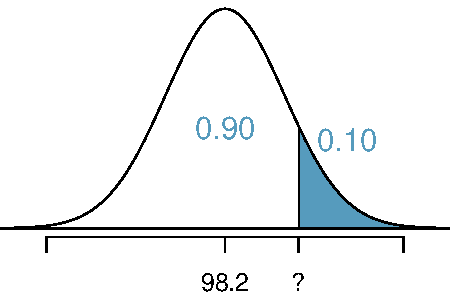
\includegraphics[width=\textwidth]{3-1_normal_distribution/tempHIGH10PERC.pdf}
}
{
\pause
{\footnotesize
\begin{tabular}{|c | rrr >{\columncolor[gray]{0.9}[0pt]}rr |}
\hline
$Z$ & 0.05 & 0.06 & 0.07 & 0.08 & 0.09 \\
  \hline
  \hline
  1.0 & \tiny{0.8531} & \tiny{0.8554} & \tiny{0.8577} & \tiny{0.8599} & \tiny{0.8621} \\
  1.1  & \tiny{0.8749} & \tiny{0.8770} & \tiny{0.8790} & \tiny{0.8810} & \tiny{0.8830} \\
   \rowcolor[gray]{.9}
 1.2 & \tiny{0.8944} & \tiny{0.8962} & \tiny{0.8980} & \tiny{\orange{0.8997}} & \tiny{0.9015} \\
  1.3 & \tiny{0.9115} & \tiny{0.9131} & \tiny{0.9147} & \tiny{0.9162} & \tiny{0.9177} \\
   \hline
\end{tabular}
}
}
}
\pause
\scalefont{0.6}
\begin{eqnarray*}
P(X > x) &=& 0.10 \rightarrow P(Z < \orange{1.28}) = 0.90 \\ \pause
Z &=& \frac{obs~-~media}{SD} \rightarrow \frac{x - 98.2}{0.73} = 1.28 \\ \pause
x &=& (1.28 \times 0.73) + 98.2 = 99.1
\end{eqnarray*}

\end{frame}

%%%%%%%%%%%%%%%%%%%%%%%%%%%%%%%%%%%%

\subsection{Regra 68-95-99.7}

%%%%%%%%%%%%%%%%%%%%%%%%%%%%%%%%%%%%

\begin{frame}
\frametitle{Regra 68-95-99.7}

\begin{itemize}
\justifying
\item Para dados quase normalmente distribuídos, 
\begin{itemize}
\justifying
\item cerca de 68 \% cai dentro de 1 SD da média,
\justifying
\item cerca de 95 \% cai dentro de 2 SD da média,
\justifying
\item cerca de 99,7 \% cai dentro de 3 SD da média.
\end{itemize}
\justifying
\item É possível que as observações caiam 4, 5 ou mais desvios-padrão da média, mas essas ocorrências são muito raras se os dados forem quase normais.

\end{itemize}

\begin{center}
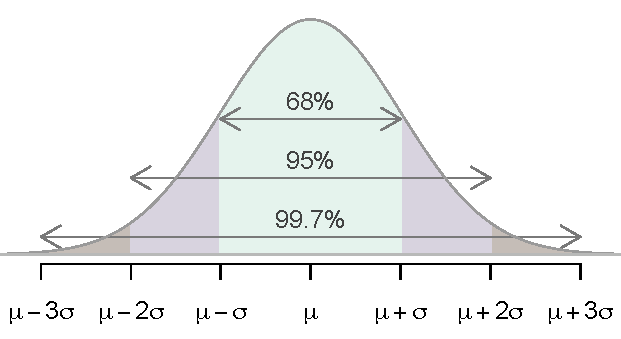
\includegraphics[width=0.7\textwidth]{3-1_normal_distribution/6895997.pdf}
\end{center}

\end{frame}

%%%%%%%%%%%%%%%%%%%%%%%%%%%%%%%%%%%%

\begin{frame}
\frametitle{Descrevendo a variabilidade usando a regra 68-95-99.7}
\justifying
Os escores do SAT são distribuídos quase que normalmente com média 1.500 e desvio padrão 300.

\pause
\begin{itemize}
\justifying
\footnotesize
\item $\sim$68\% dos alunos possuem pontuação entre 1200 e 1800 no SAT.
\justifying
\item $\sim$95\% dos alunos possuem pontuação entre 900 e 2100 no SAT. 
\justifying
\item $\sim$99.7\% dos alunos possuem pontuação entre 600 e 2400 no SAT. 

\end{itemize}

\begin{center}
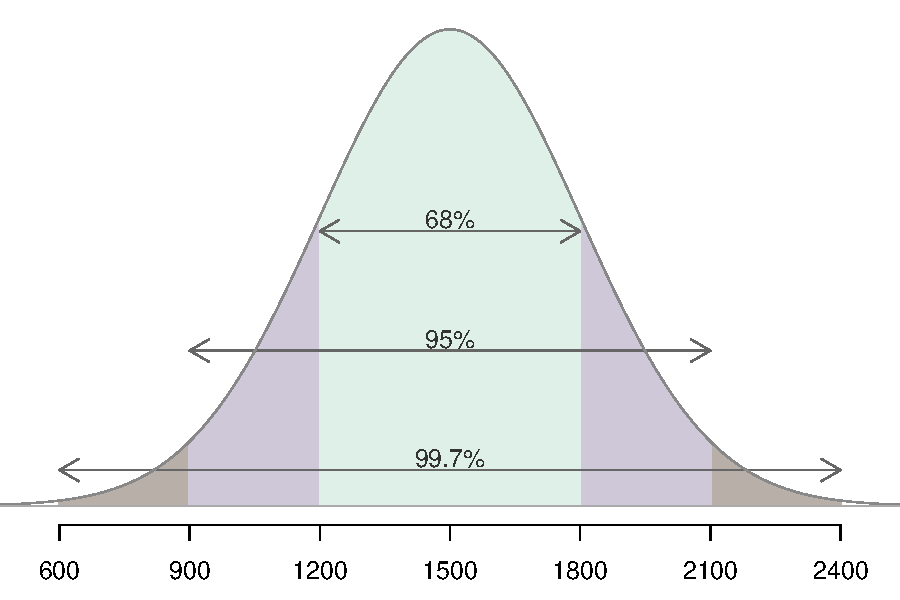
\includegraphics[width=0.65\textwidth]{3-1_normal_distribution/sat_empirical.pdf}
\end{center}

\end{frame}

%%%%%%%%%%%%%%%%%%%%%%%%%%%%%%%%%%%%

\begin{frame}[fragile]
\frametitle{Número de horas de sono de estudantes}

\only<1 | handout:0>{
\begin{center}
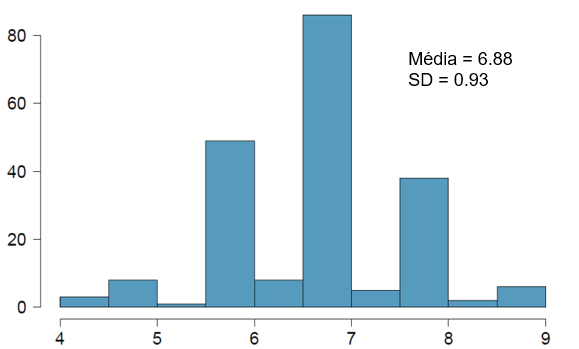
\includegraphics[width=0.75\textwidth]{3-1_normal_distribution/sleep-hist.png} 
\end{center}
\vspace{-0.25cm}
\begin{itemize}
\item Média = 6.88 horas, SD = 0.92 horas
\item[] \textcolor{white}{72\% dos dados estão dentro de 1 SD da média: $6.88 \pm 0.93$}
\item[] \textcolor{white}{92\% dos dados estão dentro de 1 SD da média: $6.88 \pm 2 \times 0.93$}
\item[] \textcolor{white}{99\% dos dados estão dentro de 1 SD da média: $6.88 \pm 3 \times 0.93$}
\end{itemize}
}

\only<2 | handout:0>{
\begin{center}
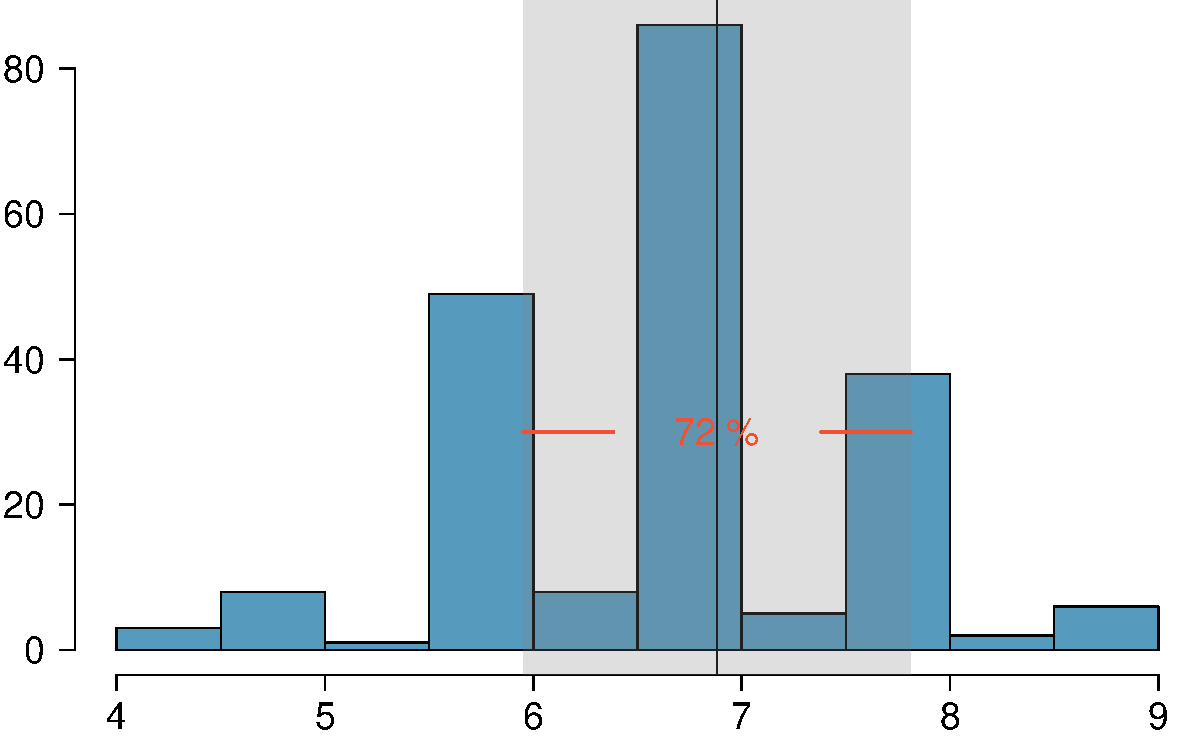
\includegraphics[width=0.75\textwidth]{3-1_normal_distribution/sleep-hist-sd1.pdf} 
\end{center}
\vspace{-0.25cm}
\begin{itemize}
\justifying
\item Média = 6.88 horas, SD = 0.92 horas
\justifying
\item 72\% dos dados estão dentro de 1 SD da média: $6.88 \pm 0.93$
\justifying
\item[] \textcolor{white}{92\% dos dados estão dentro de 1 SD da média: $6.88 \pm 2 \times 0.93$}
\justifying
\item[] \textcolor{white}{99\% dos dados estão dentro de 1 SD da média: $6.88 \pm 3 \times 0.93$}
\end{itemize}
}

\only<3 | handout:0>{
\begin{center}
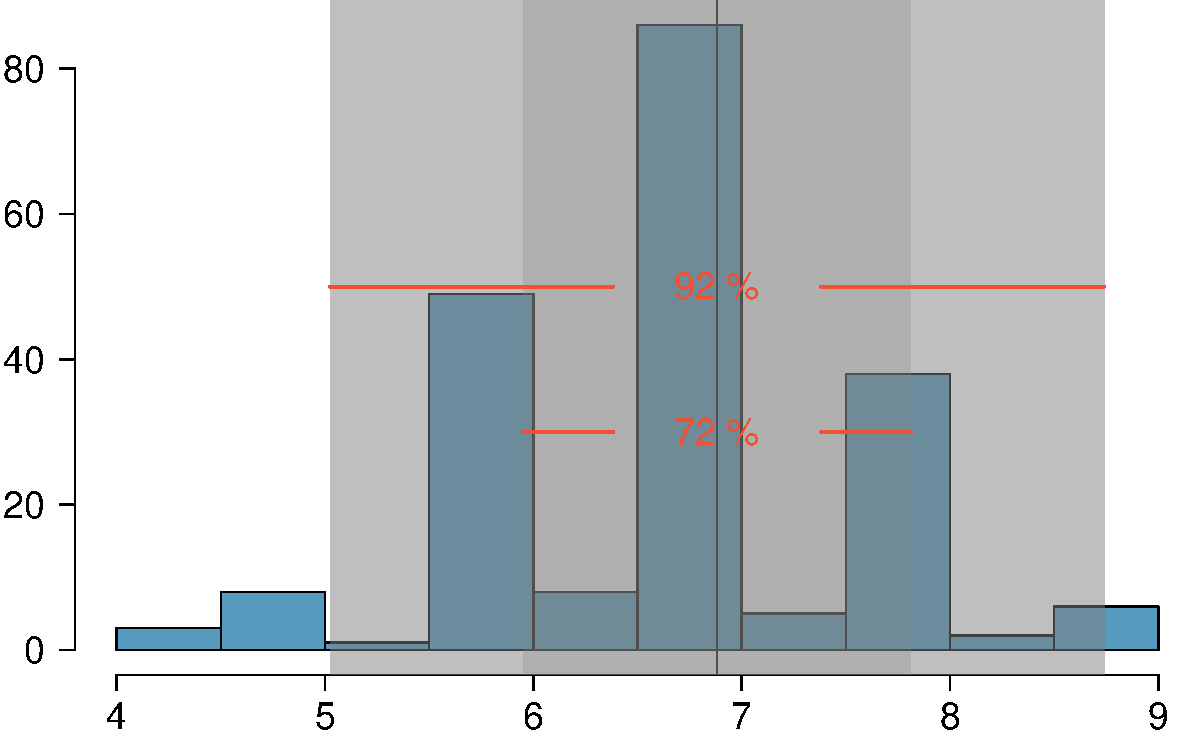
\includegraphics[width=0.75\textwidth]{3-1_normal_distribution/sleep-hist-sd2.pdf} 
\end{center}
\vspace{-0.25cm}
\begin{itemize}
\justifying
\item Média = 6.88 horas, SD = 0.92 horas
\justifying
\item 72\% dos dados estão dentro de 1 SD da média: $6.88 \pm 0.93$
\justifying
\item 92\% dos dados estão dentro de 1 SD da média: $6.88 \pm 2 \times 0.93$
\justifying
\item[] \textcolor{white}{99\% dos dados estão dentro de 1 SD da média: $6.88 \pm 3 \times 0.93$}
\end{itemize}
}

\only<4>{
\begin{center}
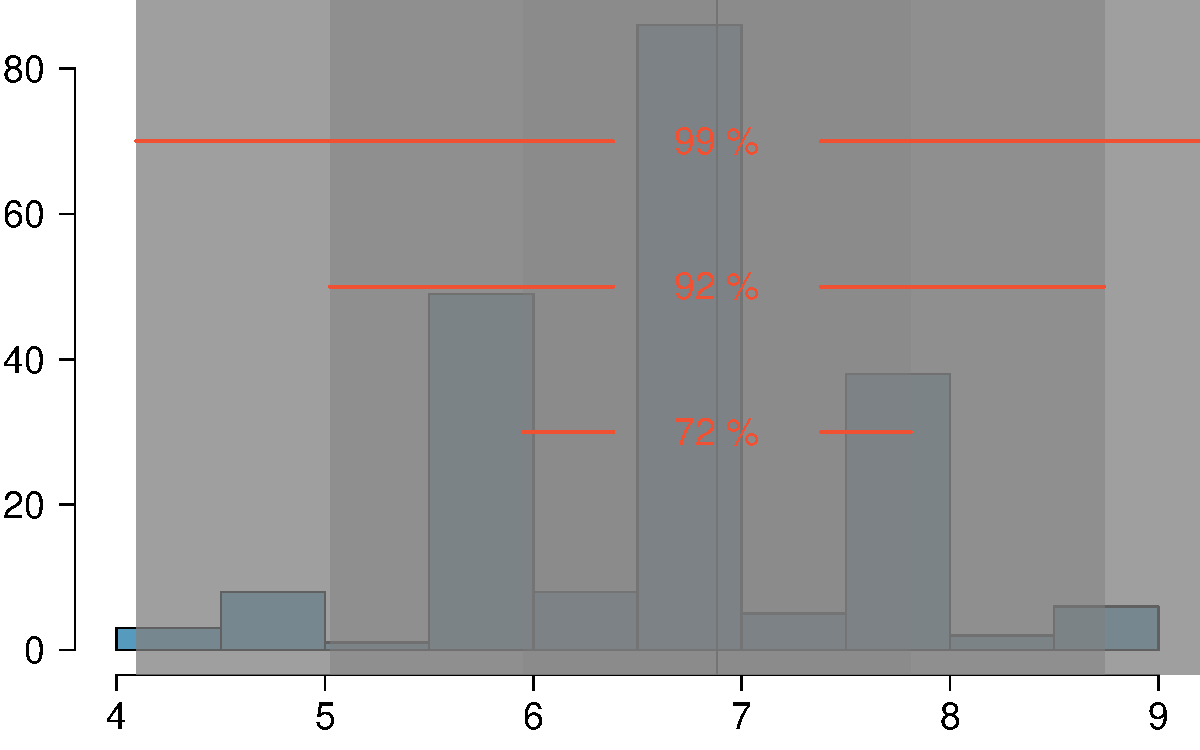
\includegraphics[width=0.75\textwidth]{3-1_normal_distribution/sleep-hist-sd3.pdf} 
\end{center}
\vspace{-0.2cm}
\small{
\begin{itemize}
\justifying
\item Média = 6.88 horas, SD = 0.92 horas
\justifying
\item 72\% dos dados estão dentro de 1 SD da média: $6.88 \pm 0.93$
\justifying
\item 92\% dos dados estão dentro de 1 SD da média: $6.88 \pm 2 \times 0.93$
\justifying
\item 99\% dos dados estão dentro de 1 SD da média: $6.88 \pm 3 \times 0.93$
\end{itemize}
}}

\end{frame}

%%%%%%%%%%%%%%%%%%%%%%%%%%%%%%%%%%%%

\begin{frame}
\frametitle{Prática}
\justifying
\pq{Qual das seguintes opções é \underline{falsa}?}

\begin{enumerate}[(a)]
\justifying
\item A maioria dos escores Z de uma distribuição assimétrica à direita são negativos.
\justifying
\solnMult{Em distribuições assimétricas, o escore Z da média pode ser diferente de 0.}
\justifying
\item Para uma distribuição normal, o IQR é inferior a $2 \times SD$.
\justifying
\item Os escores Z são úteis para determinar o quão incomum é um ponto de dados quando comparado ao restante dos dados da distribuição.
\end{enumerate}

\end{frame}

%%%%%%%%%%%%%%%%%%%%%%%%%%%%%%%%%%%%

